%%%%%%%%%%%%%%%%%%%%%%%%%%%%%%%%%%%%%%%%%%%%%%%%%%%%%%%%%%%%%%%%%%%%%%%%%%%%%%%
\documentclass[12pt]{report}

%%%%%%%%%%%%%%%%%%%%%%%%%%%%%%%%%%%%%%%%%%%%%%%%%%%%%%%%%%%%%%%%%%%%%%%%%%%%%%%
% PACKAGES
%%%%%%%%%%%%%%%%%%%%%%%%%%%%%%%%%%%%%%%%%%%%%%%%%%%%%%%%%%%%%%%%%%%%%%%%%%%%%%%

% package for projects with multiple files
\usepackage{subfiles}

% formatting packages
\usepackage[
    left=1.5in,     % left margin
    right=1.0in,    % right margin
    top=1.0in,      % top margin
    bottom=1.0in,   % bottom margin
    includefoot     % page number does not protrude into bottom margin
    ]{geometry}     % set margins
\usepackage{titlesec}	                    % custom section titles
\usepackage{appendix}                       % customizable appendices
\usepackage{caption}                        % table and figure captions
\usepackage[nodisplayskipstretch]{setspace} % double spacing
\usepackage[hidelinks]{hyperref} 	        % clickable links/toc
\usepackage[titles]{tocloft}                % table of contents extension
\usepackage[sectionbib]{bibunits}           % separate bib by chapter
\usepackage[
    section,    % bibliographies are sections, not chapters
    numbib,     % bibliographies are numbered
    nottoc,     % do not change table of contents
    notlof,     % do not change list of figures
    notlot,     % do not change list of tables
    ]{tocbibind} % include bibliographies in table of contents

% symbol packages
\usepackage{amsmath}
\usepackage{amsthm}
\usepackage{amssymb}
\usepackage{mathtools}
\usepackage{stmaryrd}

% tables and lists
\usepackage{enumerate}
\usepackage{array}
\usepackage{tabularx}
\usepackage{multirow}
\usepackage{dcolumn}

% images and figures
\usepackage[dvips,dvipdf]{graphicx}

% additional packages (uncomment/add as needed)
\usepackage[usenames,dvipsnames]{color}
\usepackage{lipsum}

%%%%%%%%%%%%%%%%%%%%%%%%%%%%%%%%%%%%%%%%%%%%%%%%%%%%%%%%%%%%%%%%%%%%%%%%%%%%%%%
% FORMATTING
%%%%%%%%%%%%%%%%%%%%%%%%%%%%%%%%%%%%%%%%%%%%%%%%%%%%%%%%%%%%%%%%%%%%%%%%%%%%%%%

% chapter, section, subsection titles
\titleformat{\chapter}[hang]{\bfseries\normalsize\centering}{\thechapter.}{5pt}{}[]
\titleformat{\section}[hang]{\bfseries}{\thesection.}{5pt}{}[]
\titleformat{\subsection}[runin]{\bfseries}{\thesubsection.}{5pt}{}[:]

% front matter format
\newcommand\frontstuff[1]{
    \chapter*{#1}
    \addcontentsline{toc}{chapter}{#1}
}

% add periods to numbers in toc
\let \savenumberline \numberline
\def \numberline#1{\savenumberline{#1.}}

% add dots to toc (from name to page number)
\renewcommand{\cftchapleader}{\cftdotfill{\cftdotsep}}

% bibliography name and style
\renewcommand{\bibname}{References}
\defaultbibliographystyle{abbrv}

% set caption font size
\captionsetup[figure]{font=footnotesize,labelfont=footnotesize}
\captionsetup[table]{font=footnotesize,labelfont=footnotesize}

%%%%%%%%%%%%%%%%%%%%%%%%%%%%%%%%%%%%%%%%%%%%%%%%%%%%%%%%%%%%%%%%%%%%%%%%%%%%%%%
% MACROS
%%%%%%%%%%%%%%%%%%%%%%%%%%%%%%%%%%%%%%%%%%%%%%%%%%%%%%%%%%%%%%%%%%%%%%%%%%%%%%%

% https://github.com/samreynoldsmath/texmf
%%%%%%%%%%%%%%%%%%%%%%%%%%%%%%%%%%%%%%%%%%%%%%%%%%%%%%%%%%%%%%%%%%%%%%%%%%%%%%%%
% Packages
%%%%%%%%%%%%%%%%%%%%%%%%%%%%%%%%%%%%%%%%%%%%%%%%%%%%%%%%%%%%%%%%%%%%%%%%%%%%%%%%

\usepackage{amsmath}
\usepackage{amssymb}
\usepackage{mathtools}
\usepackage{stmaryrd} 			% brackets
\usepackage[new]{old-arrows} 	% arrows

%%%%%%%%%%%%%%%%%%%%%%%%%%%%%%%%%%%%%%%%%%%%%%%%%%%%%%%%%%%%%%%%%%%%%%%%%%%%%%%%
% Equation Environments
%%%%%%%%%%%%%%%%%%%%%%%%%%%%%%%%%%%%%%%%%%%%%%%%%%%%%%%%%%%%%%%%%%%%%%%%%%%%%%%%
\newcommand\eqn[1]{
	\begin{align*}
		#1
	\end{align*}
}

\newcommand\labeqn[1]{
	\begin{align}
		#1
	\end{align}
}

\newcommand\bracegroup[1]{
	\left\{
	\begin{aligned}
		#1
	\end{aligned}
	\right.
}

\newcommand\bracketgroup[1]{
	\left[
	\begin{aligned}
		#1
	\end{aligned}
	\right.
}

%%%%%%%%%%%%%%%%%%%%%%%%%%%%%%%%%%%%%%%%%%%%%%%%%%%%%%%%%%%%%%%%%%%%%%%%%%%%%%%%
% Text Fonts
%%%%%%%%%%%%%%%%%%%%%%%%%%%%%%%%%%%%%%%%%%%%%%%%%%%%%%%%%%%%%%%%%%%%%%%%%%%%%%%%
\newcommand\tbf{\textbf}		% text bold
\newcommand\mono{\texttt}		% fixed width
\newcommand\ul{\underline}		% underlined

%%%%%%%%%%%%%%%%%%%%%%%%%%%%%%%%%%%%%%%%%%%%%%%%%%%%%%%%%%%%%%%%%%%%%%%%%%%%%%%%
% Math Fonts
%%%%%%%%%%%%%%%%%%%%%%%%%%%%%%%%%%%%%%%%%%%%%%%%%%%%%%%%%%%%%%%%%%%%%%%%%%%%%%%%
\renewcommand\bf{\boldsymbol} 	% math bold
\newcommand\bb{\mathbb} 		% blackboard bold
\renewcommand\cal{\mathcal}		% calligraphic
\renewcommand\bar{\overline}	% overline

%%%%%%%%%%%%%%%%%%%%%%%%%%%%%%%%%%%%%%%%%%%%%%%%%%%%%%%%%%%%%%%%%%%%%%%%%%%%%%%%
% Special Letters and Symbols
%%%%%%%%%%%%%%%%%%%%%%%%%%%%%%%%%%%%%%%%%%%%%%%%%%%%%%%%%%%%%%%%%%%%%%%%%%%%%%%%
\newcommand{\eps}{\varepsilon}	% curvy epsilon
\newcommand{\phii}{\varphi} 	% curvy phi

%%%%%%%%%%%%%%%%%%%%%%%%%%%%%%%%%%%%%%%%%%%%%%%%%%%%%%%%%%%%%%%%%%%%%%%%%%%%%%%%
% Hats and Tildes
%%%%%%%%%%%%%%%%%%%%%%%%%%%%%%%%%%%%%%%%%%%%%%%%%%%%%%%%%%%%%%%%%%%%%%%%%%%%%%%%
\renewcommand\hat\widehat
\renewcommand\tilde\widetilde

%%%%%%%%%%%%%%%%%%%%%%%%%%%%%%%%%%%%%%%%%%%%%%%%%%%%%%%%%%%%%%%%%%%%%%%%%%%%%%%%
% Brackets, Braces, and Bars
%%%%%%%%%%%%%%%%%%%%%%%%%%%%%%%%%%%%%%%%%%%%%%%%%%%%%%%%%%%%%%%%%%%%%%%%%%%%%%%%
\newcommand{\DeclareAutoPairedDelimiter}[3]{
	\expandafter\DeclarePairedDelimiter\csname Auto\string#1\endcsname{#2}{#3}
	\DeclareRobustCommand{#1}{\csname Auto\string#1\endcsname*}}

\DeclareAutoPairedDelimiter{\paren}{ ( }{ ) }			% parentheses
\DeclareAutoPairedDelimiter{\bracket}{ [ }{ ] }			% square brackets
\DeclareAutoPairedDelimiter{\curly}{ \{ }{ \} }			% curly braces
\DeclareAutoPairedDelimiter{\abs}{|}{|}					% absolute value
\DeclareAutoPairedDelimiter{\norm}{\|}{\|}				% norm
\DeclareAutoPairedDelimiter{\ip}{\langle}{\rangle}		% inner product
\DeclareAutoPairedDelimiter{\ceil}{\lceil}{\rceil} 		% ceiling
\DeclareAutoPairedDelimiter{\floor}{\lfloor}{\rfloor} 	% floor

%%%%%%%%%%%%%%%%%%%%%%%%%%%%%%%%%%%%%%%%%%%%%%%%%%%%%%%%%%%%%%%%%%%%%%%%%%%%%%%%
% Special Sets
%%%%%%%%%%%%%%%%%%%%%%%%%%%%%%%%%%%%%%%%%%%%%%%%%%%%%%%%%%%%%%%%%%%%%%%%%%%%%%%%
\newcommand{\nada}{\varnothing} % empty set
\newcommand{\C}{\mathbb{C}}		% complex plane
\newcommand{\F}{\mathbb{F}}		% arbitrary field
\newcommand{\K}{\mathbb{K}}		% arbitrary field
\newcommand{\N}{\mathbb{N}}		% natural numbers
\renewcommand{\P}{\mathbb{P}}		% polynomials
\newcommand{\Q}{\mathbb{Q}}		% rationals
\newcommand{\R}{\mathbb{R}}		% reals
\newcommand{\Z}{\mathbb{Z}}		% integers

%%%%%%%%%%%%%%%%%%%%%%%%%%%%%%%%%%%%%%%%%%%%%%%%%%%%%%%%%%%%%%%%%%%%%%%%%%%%%%%%
% Relations
%%%%%%%%%%%%%%%%%%%%%%%%%%%%%%%%%%%%%%%%%%%%%%%%%%%%%%%%%%%%%%%%%%%%%%%%%%%%%%%%

% open subset symbol: \subset + \circ (Thank you, Jay!)
\DeclareFontEncoding{LS1}{}{}
\DeclareFontSubstitution{LS1}{stix}{m}{n}
\DeclareSymbolFont{symbols2}      {LS1}{stixfrak} {m} {n}
\DeclareMathSymbol{\subsetocirc}{\mathord}{symbols2}{"05}
\newcommand{\subseto}{\mathop{\,\subsetocirc\,}}

%%%%%%%%%%%%%%%%%%%%%%%%%%%%%%%%%%%%%%%%%%%%%%%%%%%%%%%%%%%%%%%%%%%%%%%%%%%%%%%%
% Algebra
%%%%%%%%%%%%%%%%%%%%%%%%%%%%%%%%%%%%%%%%%%%%%%%%%%%%%%%%%%%%%%%%%%%%%%%%%%%%%%%%
\newcommand\inv{^{-1}} % inverse

%%%%%%%%%%%%%%%%%%%%%%%%%%%%%%%%%%%%%%%%%%%%%%%%%%%%%%%%%%%%%%%%%%%%%%%%%%%%%%%%
% Complex Analysis
%%%%%%%%%%%%%%%%%%%%%%%%%%%%%%%%%%%%%%%%%%%%%%%%%%%%%%%%%%%%%%%%%%%%%%%%%%%%%%%%
\newcommand{\ii}{\mathfrak{i}} 	% complex i
\renewcommand\Re{\text{Re}\,}
\renewcommand\Im{\text{Im}\,}

%%%%%%%%%%%%%%%%%%%%%%%%%%%%%%%%%%%%%%%%%%%%%%%%%%%%%%%%%%%%%%%%%%%%%%%%%%%%%%%%
% Matrices
%%%%%%%%%%%%%%%%%%%%%%%%%%%%%%%%%%%%%%%%%%%%%%%%%%%%%%%%%%%%%%%%%%%%%%%%%%%%%%%%
\newcommand{\pmat}[1]{\begin{pmatrix}#1\end{pmatrix}} % soft
\newcommand{\bmat}[1]{\begin{bmatrix}#1\end{bmatrix}} % hard

%%%%%%%%%%%%%%%%%%%%%%%%%%%%%%%%%%%%%%%%%%%%%%%%%%%%%%%%%%%%%%%%%%%%%%%%%%%%%%%%
% Linear Algebra
%%%%%%%%%%%%%%%%%%%%%%%%%%%%%%%%%%%%%%%%%%%%%%%%%%%%%%%%%%%%%%%%%%%%%%%%%%%%%%%%

\renewcommand\t{^\intercal} 			% transpose
\newcommand\invt{^{-\intercal}} 		% inverse transpose
\newcommand\spn{\operatorname{span}} 	% span
\newcommand\range{\operatorname{range}}	% range
\newcommand\nul{\operatorname{null}} 	% null space
\newcommand\rank{\operatorname{rank}} 	% rank
\newcommand\tr{\operatorname{tr}} 	% trace
\newcommand\trace\tr
\newcommand\diag{\operatorname{diag}}	% diagonal

%%%%%%%%%%%%%%%%%%%%%%%%%%%%%%%%%%%%%%%%%%%%%%%%%%%%%%%%%%%%%%%%%%%%%%%%%%%%%%%%
% Calculus
%%%%%%%%%%%%%%%%%%%%%%%%%%%%%%%%%%%%%%%%%%%%%%%%%%%%%%%%%%%%%%%%%%%%%%%%%%%%%%%%

\renewcommand{\div}{\operatorname{div}}
\DeclareMathOperator{\grad}{grad} % gradient
\DeclareMathOperator{\curl}{curl}	% curl
\newcommand\pdd[2]{\dfrac{\partial #1}{\partial #2}} % partial derivative
\newcommand\pd[2]{\frac{\partial #1}{\partial #2}} % partial derivative
\newcommand\nd[1]{\frac{\partial #1}{\partial\bf{n}}} % normal derivative
\newcommand\td[1]{\frac{\partial #1}{\partial\bf{t}}} % tangential derivative

%%%%%%%%%%%%%%%%%%%%%%%%%%%%%%%%%%%%%%%%%%%%%%%%%%%%%%%%%%%%%%%%%%%%%%%%%%%%%%%%
% Analysis
%%%%%%%%%%%%%%%%%%%%%%%%%%%%%%%%%%%%%%%%%%%%%%%%%%%%%%%%%%%%%%%%%%%%%%%%%%%%%%%%

\DeclareMathOperator*{\esssup}{ess\,sup}
\DeclareMathOperator{\weakto}{\rightharpoonup}
\DeclareMathOperator*{\embed}{\longhookrightarrow}
\DeclareMathOperator{\dom}{dom}

%%%%%%%%%%%%%%%%%%%%%%%%%%%%%%%%%%%%%%%%%%%%%%%%%%%%%%%%%%%%%%%%%%%%%%%%%%%%%%%%
% Optimization
%%%%%%%%%%%%%%%%%%%%%%%%%%%%%%%%%%%%%%%%%%%%%%%%%%%%%%%%%%%%%%%%%%%%%%%%%%%%%%%%

\newcommand\st{\text{st}\;}
\newcommand\psdcone{S^n_+}
\newcommand\aff{\text{aff}\;}

%%%%%%%%%%%%%%%%%%%%%%%%%%%%%%%%%%%%%%%%%%%%%%%%%%%%%%%%%%%%%%%%%%%%%%%%%%%%%%%%
% Geometry
%%%%%%%%%%%%%%%%%%%%%%%%%%%%%%%%%%%%%%%%%%%%%%%%%%%%%%%%%%%%%%%%%%%%%%%%%%%%%%%%

\DeclareMathOperator*{\diam}{diam}

%%%%%%%%%%%%%%%%%%%%%%%%%%%%%%%%%%%%%%%%%%%%%%%%%%%%%%%%%%%%%%%%%%%%%%%%%%%%%%%%
% Messages
%%%%%%%%%%%%%%%%%%%%%%%%%%%%%%%%%%%%%%%%%%%%%%%%%%%%%%%%%%%%%%%%%%%%%%%%%%%%%%%%

\newcommand\goodbye{So long, farewell, Auf Wiedersehen, goodbye!}

\usepackage{preamble/chapterheader}

\newcommand\PSU{Fariborz Maseeh Department of Mathematics and Statistics,
Portland State University, Portland, OR 97201}

\makeatletter
\newcommand\footnoteref[1]{\protected@xdef\@thefnmark{\ref{#1}}\@footnotemark}
\makeatother

%%%%%%%%%%%%%%%%%%%%%%%%%%%%%%%%%%%%%%%%%%%%%%%%%%%%%%%%%%%%%%%%%%%%%%%%%%%%%%%
% THEOREM ENVIRONMENTS
%%%%%%%%%%%%%%%%%%%%%%%%%%%%%%%%%%%%%%%%%%%%%%%%%%%%%%%%%%%%%%%%%%%%%%%%%%%%%%%

% https://github.com/samreynoldsmath/texmf
\def\theoremnumberstyle{chaptersection}
\input{sams-theorems.tex}

%%%%%%%%%%%%%%%%%%%%%%%%%%%%%%%%%%%%%%%%%%%%%%%%%%%%%%%%%%%%%%%%%%%%%%%%%%%%%%%
% TITLEPAGE
%%%%%%%%%%%%%%%%%%%%%%%%%%%%%%%%%%%%%%%%%%%%%%%%%%%%%%%%%%%%%%%%%%%%%%%%%%%%%%%

\begin{document}

% help prevent text from jutting into margins
\sloppy

% due to bibunits package
\bibliographyunit[\chapter]

% no page number on title page
\pagenumbering{gobble}

% title page content
\def\AUTHOR{Guy Fieri}

\def\TITLE{
    Applications of Mustard Polynomials to Algebraic Hotdog Theory
}

\def\DEGREE{
    Doctor of Philosophy\\
    in\\
    Mathematical Sciences
}

\def\COMMITTEE{
    Rachel Ray, Chair\\
    Gordon Ramsay\\
    Paula Dean\\
    Alton Brown
}

\def\INSTITUTION{Portland State University}

\def\YEAR{2024}

% title page
\begin{center}
    \TITLE\\[1.0in]
    by\\[12pt]
    \AUTHOR
    \\[1.0in]
    A dissertation submitted in partial fulfillment of the \\
    requirements for the degree of
    \\[1.0in]
    \DEGREE
    \\[1.0in]
    Dissertation committee:\\
    \COMMITTEE\\[1.0in]
    \INSTITUTION\\
    \YEAR
\end{center}

%%%%%%%%%%%%%%%%%%%%%%%%%%%%%%%%%%%%%%%%%%%%%%%%%%%%%%%%%%%%%%%%%%%%%%%%%%%%%%%
% FRONT MATTER
%%%%%%%%%%%%%%%%%%%%%%%%%%%%%%%%%%%%%%%%%%%%%%%%%%%%%%%%%%%%%%%%%%%%%%%%%%%%%%%

\pagebreak
\pagenumbering{roman}
\doublespacing

\frontstuff{Abstract}
\lipsum[1]

\frontstuff{Dedication}
\begin{center}
    For Mum and Pop
\end{center}

\frontstuff{Acknowledgements}
Some heartfelt thanks to all the people who were helpful. Don't forget to acknowledge funding! \lipsum[1]

% table of contents
\singlespacing
\tableofcontents

% list of figures
\cleardoublepage
\phantomsection
\addcontentsline{toc}{chapter}{\listfigurename}
\listoffigures

% list of tables
\cleardoublepage
\phantomsection
\addcontentsline{toc}{chapter}{\listtablename}
\listoftables

\doublespacing

%%%%%%%%%%%%%%%%%%%%%%%%%%%%%%%%%%%%%%%%%%%%%%%%%%%%%%%%%%%%%%%%%%%%%%%%%%%%%%%
% MAIN BODY
%%%%%%%%%%%%%%%%%%%%%%%%%%%%%%%%%%%%%%%%%%%%%%%%%%%%%%%%%%%%%%%%%%%%%%%%%%%%%%%

\chapter{Introduction}
    % for first chapter only
    \pagenumbering{arabic}

    \section{Preliminaries}
        \label{introduction-preliminaries}
        \lipsum[4]

    \section{Structure of This Dissertation}
        \label{introduction-structure}
        \lipsum[3]
\chapter{Equivalence of Hot Dogs and Tacos Under Boyardee's Criterion}
\label{paper1}

% chapter heading page
\subsection*{Full citation information}
  \begin{quote}
    Jeffrey S. Ovall and Samuel E. Reynolds.
    A high-order method for evaluating derivatives of harmonic functions in planar domains.
    \textit{SIAM Journal on Scientific Computing}, 40(3):A1915--A1935, 2018.
  \end{quote}

\subsection*{Authors}
  \textit{Jeffrey S. Ovall\footnote{\label{PSU-affil-1}\PSU} and
  Samuel E. Reynolds\footnoteref{PSU-affil-1}}

\subsection*{Author contribution statement}
  \begin{itemize}
    \item Jeffrey S. Ovall:  developed algorithms, drafted the paper
    \item Samuel E. Reynolds: implemented numerical examples, investigation, review and editing
  \end{itemize}

\subsection*{DOI}
  \href{https://doi.org/10.1137/17M1141825}{10.1137/17M1141825}

\subsection*{Hyperlink to the publication in PDXScholar}
  \begin{quote}
    \url{https://archives.pdx.edu/ds/psu/26690}
  \end{quote}

\subsection*{Additional information}
  Ovall was partially supported by the NSF Grant DMS-1414365.

% content of paper
\section*{Abstract}
  \lipsum[1]

\section{Introduction}
  \lipsum[1]
  Let's cite a paper \cite{BankCVS2011}.

\section{Main Results}
  \lipsum[4]
  Another paper we can cite \cite{Babuska1996}.

  \subsection{This is a subsection}
  \lipsum[1]

  \begin{figure}
    \centering
    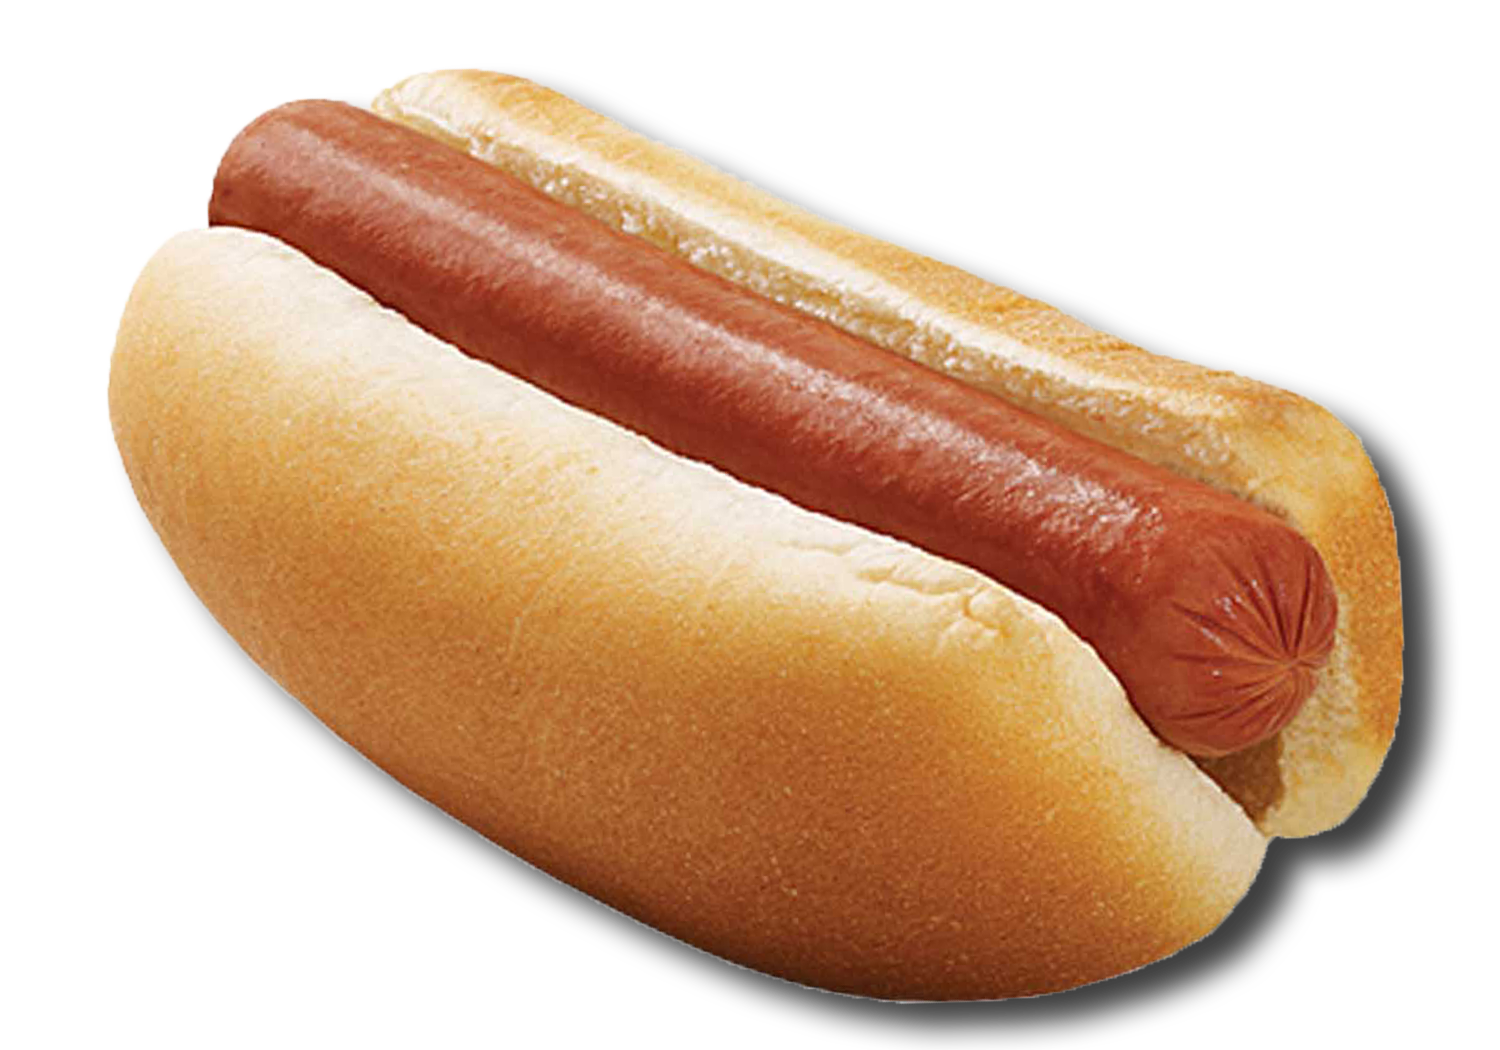
\includegraphics[width=0.4\textwidth]{src/paper1/figs/hotdog.png}
    \caption{O caption, my caption!}
  \end{figure}

  \lipsum[2]

\section{Conclusion}
  \lipsum[2]



% chapter references
\pagebreak
\singlespacing
\putbib[src/paper1/titles1]
\doublespacing

\chapter{Mustard Polynomials}
\label{paper2}

% chapter heading page
\input{src/paper1/heading2.tex}
\break

% content of paper
\section*{Abstract}
  \lipsum[1]

\section{Introduction}
  \lipsum[2]
  Let's cite this one paper \cite{Greenbaum1993}.

\section{Main Results}
  \lipsum[1]
  Now let's cite this other paper \cite{Fix1973}.

  \begin{figure}
    \centering
    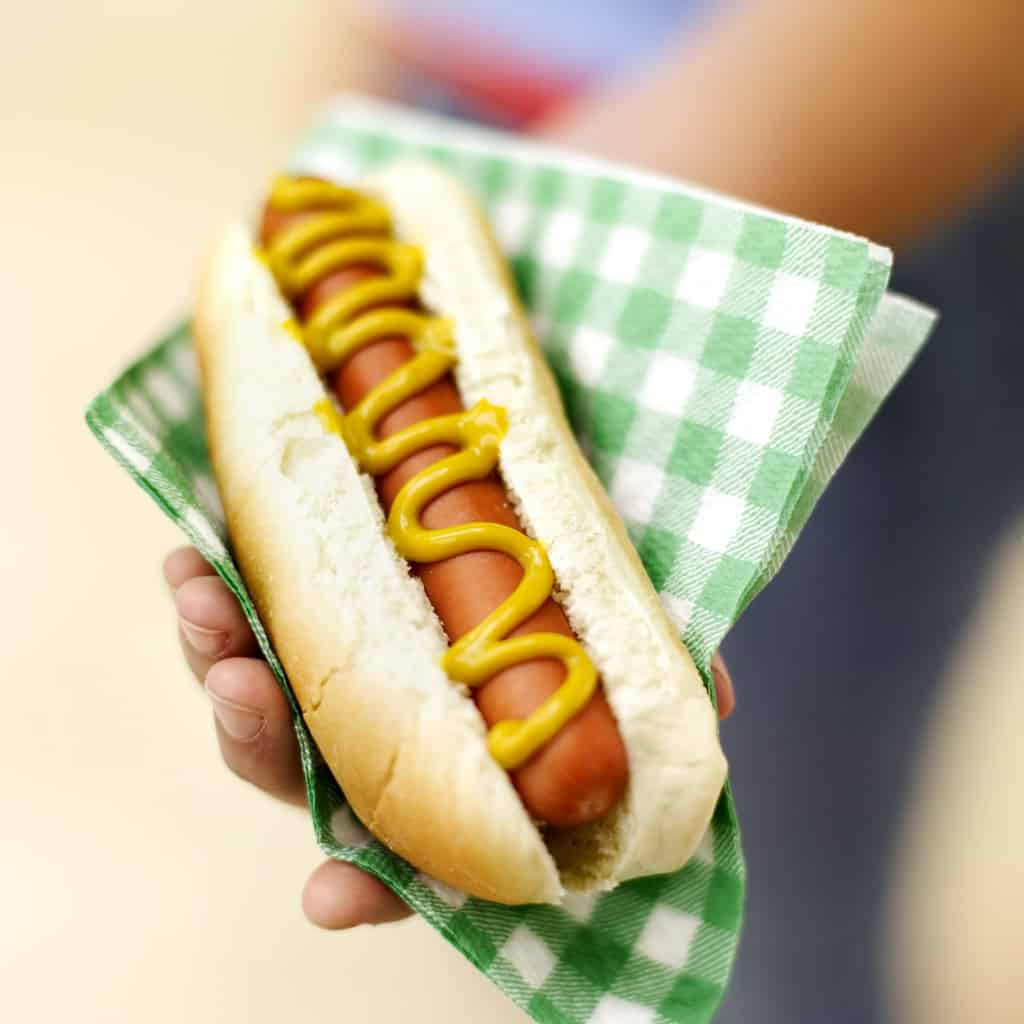
\includegraphics[width=0.4\textwidth]{src/paper2/figs/hotdog2.jpg}
    \caption{Mustard on a hot dog.}
  \end{figure}

  \lipsum[3]

  \begin{table}
    \centering
    \caption{Mustard and relish distributions.}
    \begin{tabular}{c|c|c}
      Mustard   &Relish   &Flavor \\
      \hline
      1   & 2   & $-1/12$ \\
      3   & 4   & 1.12e-3
    \end{tabular}
  \end{table}

\section{Conclusion}
  \lipsum[2]

% chapter references
\break
\singlespacing
\putbib[src/paper2/titles2]
\doublespacing

\chapter{Conclusion}
    \label{ch-conclusion}

\section{Summary}
    \label{conclusion-summary}
    \lipsum[3]

\section{Future Work}
    \label{conclusion-future-work}
    \lipsum[3]

%%%%%%%%%%%%%%%%%%%%%%%%%%%%%%%%%%%%%%%%%%%%%%%%%%%%%%%%%%%%%%%%%%%%%%%%%%%%%%%
% APPENDIX
%%%%%%%%%%%%%%%%%%%%%%%%%%%%%%%%%%%%%%%%%%%%%%%%%%%%%%%%%%%%%%%%%%%%%%%%%%%%%%%

% exclude appendix from lists of tables and figures
\let\svaddcontentsline\addcontentsline
\renewcommand\addcontentsline[3]{%
  \ifthenelse{\equal{#1}{lof}}{}%
  {\ifthenelse{\equal{#1}{lot}}{}{\svaddcontentsline{#1}{#2}{#3}}}}

% add the "Appendix" to the appendix titles
\titleformat{\chapter}[hang]{\bfseries\normalsize\centering}{Appendix \thechapter.}{5pt}{}[]
\renewcommand{\appendixname}{Appendix}
\appendixtitleon    % puts \appendixname before each appendix title
\appendixtitletocon % puts \appendixname before each TOC entry

\begin{appendices}
    \chapter{Extensions}
\label{ch-extensions}

\section{Mayo Monomials}
    \label{extensions-advection}
    \lipsum[2]

\section{Corn Dogs}
    \label{extensions-diffusion}
    \lipsum[2]

\end{appendices}

%%%%%%%%%%%%%%%%%%%%%%%%%%%%%%%%%%%%%%%%%%%%%%%%%%%%%%%%%%%%%%%%%%%%%%%%%%%%%%%
\end{document}
